\documentclass[article]{partsm}
%% need no \usepackage{Sweave.sty}
%\VignetteIndexEntry{partsm vignette}

\author{Javier L�pez-de-Lacalle \\ Universidad del Pa�s Vasco \\ \email{javlacalle@yahoo.es}}
\title{Periodic Autoregressive Time Series Models in \proglang{R}: The \pkg{partsm} Package.}
%
\Plainauthor{Javier L�pez-de-Lacalle} %% comma-separated
\Plaintitle{Periodic Autoregressive Time Series Models in R: The partsm Package.} % without formatting
\Shorttitle{Periodic Autoregressive Time Series Models in \proglang{R}: The \pkg{partsm} Package.}
%% a short title (if necessary)  % this will be the header of even pages in the document

%% an abstract and keywords
\Abstract{It is well-known that some of the macroeconomic time series display stochastic trends, moreover, when working with seasonally observed data stochastic seasonal cycles may exist as well. When these components, trend and seasonality, do not evolve independently, traditional differencing filters may not be suitable.
%Traditional time series models and seasonal adjustment methods assume that these components, trend and seasonality, are independent.
According to periodic autoregressive time series models, a seasonally varying autoregressive parameters and a periodic differencing filter are proposed for that case. %for analasying the data.

% This paper complements the standard manual pages provided by the package by carrying out an entire application,...
%
%This paper describes the functionality and use of the \pkg{partsm} \proglang{R}-package by puting into practice % applying
%the tools % ver sin�nimo tools
%implemented in the package and interpreting the results accordingly.
This paper focuses on practical issues % matters
%introduces the periodic autoregressive models and shows the use of the \pkg{partsm} \proglang{R}-package.
showing the use of the \pkg{partsm} \proglang{R}-package. This package allows the user to
% carry out the following tasks
check for periodicity in the data, fit a periodic autoregressive model of order p, PAR(p), select the periodic autoregressive lag order parameter,  test for periodic integration, fit a periodically integrated autoregressive model up to order 2, PIAR, as well as to perform out-of-sample forecasts.

% quarterly time series. Decir cu�l(es) es(son) las series de ejemplo.
}
\Keywords{Time series, PAR models, periodic integration, \proglang{R}} %% comma-separated, not capitalized
\Plainkeywords{Time series, PAR models, periodic integration, R} %% without formatting

%% Date
\Month{Setiembre}
\Year{2005}

%% The address of (at least) one author should be given
%% in the following format:
\Address{
  Javier L�pez-de-Lacalle.\\
  Universidad del Pa�s Vasco.\\
  Facultad de Ciencias Econ�micas y Empresariales.\\
  48015 Bilbao, Spain.\\
  E-mail: \email{javlacalle@yahoo.es}.\\
  URL: \url{http://www.bl.ehu.es/~jedlobej}.
}
%% It is also possible to add a telephone and fax number
%% before the e-mail in the following format:
%% Telephone: +43/1/31336-5053
%% Fax: +43/1/31336-734

%% end of declarations %%%%%%%%%%%%%%%%%%%%%%%%%%%%%%%%%%%%%%%%%%%%%%%

\begin{document}

\section[Introduction]{Introduction}

% ejemplo econ�mico de los modelos PAR pp. 92. Un modelo para cada estaci�n, se estima un poar�metro para cada estaci�n, no misma tendencia siempre. split the (quarterly) data out into four series.
It is well-known that some of the macroeconomic time series display stochastic trends, moreover, when working with seasonally observed data stochastic seasonal cycles may exist as well. When these components, trend and seasonality, do not evolve independently, traditional differencing filters may not be suitable.
%Traditional time series models and seasonal adjustment methods assume that these components, trend and seasonality, are independent.
According to periodic autoregressive time series models, a seasonally varying autoregressive parameters and a periodic differencing filter are proposed for that case. %for analasying the data. 
For a review of this literature see \citet{Franses:96}, \citet{Franses-Paap:04}, and references therein. % Franses y otro 2004 

This paper focuses on practical issues % matters
%introduces the periodic autoregressive models and shows the use of the \pkg{partsm} \proglang{R}-package.
showing the use of the \pkg{partsm} \proglang{R}-package. This package allows the user to check for periodicity in the data, fit a periodic autoregressive model of order p, PAR(p), select the periodic autoregressive lag order parameter, test for periodic integration, fit a periodically integrated autoregressive model up to order 2, PIAR, as well as to perform out-of-sample forecasts.

The remaining of the paper is organized as follows. Section \ref{Sreview} briefly reviews the statistical issues the \pkg{partsm} \proglang{R}-package is concerned, namely periodic autoregressive models and periodic integration. Section \ref{Sdesc} describes the package. Section \ref{Sexample} puts into practice the tools implemented in the package showing how to use them and interpreting the results accordingly. Some known bugs are mentioned in Section \ref{Sbugs}.

%% VER si pongo conclusiones con ToDo (cointegraci�n y m�s ra�ces unitarias) y posibles discrepancias con resultados de Franses:96     %%%%%%%

\section[Theoretical overview]{Theoretical overview} \label{Sreview}

This section reviews the main theoretical concerns entailed in the process of fitting periodic models and testing for a unit root in PAR models. To have a further insight into this models see \citet{Franses:96}, \citet{Franses-Paap:04}, and references therein. PAR models are intended for seasonally obeserved data, particularly quarterly and monthly data. To save space, hereafter we will consider quarterly data, $S=4$.

\subsection[Notation and representation of PAR models]{Notation and representation of PAR models}

The \textit{univariate representation} of a PAR(p) model is as follows,

\begin{equation}
\label{PAR}
y_t = \phi_{1s} y_{t-1} + ... + \phi_{ps} y_{t-p} + \epsilon_t, \quad \epsilon_t \sim iid (0,1),
\end{equation}
%
for $s=1,...,4$, for $t=1,2,...,n$, where $n$ is the number of observations. Hence, the autoregressive parameters vary with the season for each lag. 

Since a PAR(p) entails four different AR(p) models, one for each season, it is useful to rewrite (\ref{PAR}) as the \textit{multivariate representation} or \textit{vector of quarters representation}.
%
\begin{equation}         
\label{PARVQ}
\Phi_0\,Y_{s,T} = \Phi_1\,Y_{s,T-1} + ... + \Phi_P\,Y_{s,T-P} + \epsilon_T, \quad \epsilon_T \sim iid (0,1),
\end{equation}
%
where $\Phi_0, \Phi_1,...,\Phi_P$ are $(4\times4)$ parameter matrices with the parameters in (\ref{PAR}) as follows:
%
\begin{eqnarray*}
\Phi_0\,(i,j) &=& 1 \quad if \quad i=j \\
              &=& 0 \quad if \quad j > i \\
              &=& -\phi_{i-j,i} \quad if \quad j < y \\
\Phi_k\,(i,j) &=& \phi_{i+4k-j,i},
\end{eqnarray*}
%
for $i,j=1,2,3,4$ and $k=1,2,...,P$. The univariate model of order $p$ turns into a multivariate model of order $P=1+[(p-1)/4]$, where $[x]$ is the integer part of $x$.

Notice that in (\ref{PAR}) each lag leads to previous observations in the seasonally observed data, whereas in (\ref{PARVQ}) lags have effect on the anually observed data in each season. That is, $y_{t-1}$ is the observation inmediately previous to $y_t$, and $Y_{s,T-1}$ is the observation in season $s$ previous to the year $T$.

Finally, if the roots of the factorized AR(p) model related to each season are all real values, the PAR(p) model can be represented as
%
\begin{eqnarray}  %% VER esta ecuaci�n en 8.16 Franses:96 e incorporar m�s adelante en partsm.
y_t-\alpha_s\,y_{t-1} &=& \beta_{1s}\,(y_{t-1} - \alpha_{s-1}\,y_{t-2}) + ... + \\ \nonumber
&+& \beta_{(p-1)s}\,(y_{t-(p-1)} - \alpha_{s-(p-1)}\,y_{t-p}) + \epsilon_t, \quad \epsilon_t \sim iid (0,1).
\end{eqnarray}
%
called the \textit{periodically differenced form of} (\ref{PAR}).

\subsection[Periodic integration]{Periodic integration} \label{Sreview.pi}

Basically, a time series with a unit root, $y_t$, is periodically integrated if there exist % are 
some $\alpha_s$ for $s=1,2,...,4$, in such a way that the transformed series $(1-\alpha_s\,B)\,y_t$ does not contain a unit root, where $B$ is the backward operator. For the shake of rigurosity, %% ver rigurosity
the definition of \citet{Franses:96} is transcribed below.
%
\begin{quotation}
A quarterly time series $y_t$ is said to be \textit{periodically integrated of order 1} [PI] when the differencing filter $(1-\alpha_s\,B)$ is needed to remove the stochastic trend from $y_t$, where $\alpha_s$ are seasonally varying parameters with the property that $\alpha_1\alpha_2\alpha_3\alpha_4=1$ and $\alpha_s \neq \alpha$ for all $s=1,2,3,4$.
\end{quotation}

At present, the package \pkg{partsm} only allow to estimate periodically integrated autoregressive models up to order 2\footnote{PAR models use to be more parsimonious models and a first or second order model may be suitable for the data. In \citet{Franses:96}, only one out of the eleven series analysed required a higher order PAR model.}. Taking the periodically differenced representation, the following model can be estimated by non-linear least squares.

\begin{equation}    
\label{PIAR2}
y_t - \alpha_s y_{t-1} = \beta_s (y_{t-1} - \alpha_{s-1} y_{t-2}) + \epsilon_t, \quad \epsilon_t \sim iid (0,1),
\end{equation}
%
under the non-linear restriction $\prod_{s=1}^{4} \alpha_s = 1$ for $s=1,...,4$. Obviously, for a first order PIAR process $\beta$ parameters are equal to zero. This model can be estimated by non-linear least squares.

Note that the restriction above is fulfilled in these particular cases, among others. When $\alpha_s=1$ for $s=1,2,3,4$, and $\alpha_s=-1$ for $s=1,2,3,4$. 
%may give rise to the $(1-L)$ differencing filter, if $\alpha_s=1$ for $s=1,2,3,4$, or to the $(1+L)$ differencing filter, if $\alpha_s=-1$ for $s=1,2,3,4$.
The former case give rise to the $(1-L)$ differencing filter, whereas the latter entails the $(1+L)$ differencing filter. 
%
Therefore, the restriction may involve the long run unit root 1, or the seasonal unit root -1, or neither of them.

When the hypothesis above cannot be rejected it is said that the process is a \textit{PAR process for a I(1) times series}, PARI. Otherwise, the PAR model is known as a \textit{periodically integrated AR model}, PIAR, and the periodic differencing filter is obtained from the $\alpha_s$ estimates in equation (\ref{PIAR2}).

%%Taking this issue into account, 
%As we will make %do
%in Section \ref{Sexample}, 
%a common strategy in empirical applications is to test for the non-linear restriction $\prod_{s=1}^4\,\alpha_s=1$ and then test for the %hypotheses above\footnote{In practice, only three restrictions are checked, since $\alpha_s=1 \mbox{or} -1$ just for $s=1,2,3$ %entails either $\alpha_4=1$ or $\alpha_4=-1$.}. 
%%After checking whether periodicity in the autoregressive parameters exist,
%After checking for periodicity, in Section \ref{Sexample} we will see the corresponding statistics for carrying out this strategy.

In Section \ref{Sexample} we will see how to carry out this analysis following a common strategy for the empirical analysis. First, we will take a look at the package we will use for it.

\section[The partsm package]{The \pkg{partsm} package} \label{Sdesc}

\subsection[Description]{Description}

This section documents the \pkg{partsm} package version 1.0 built on the \proglang{R} language and environment for statistical computing and graphics \citep{Chambers:98, Rproject}. The package performs some of the relevant tests and models for fitting periodic autoregressive time series model introduced in the previous section.

The package is distributed under the General Public License [GPL] version 2 or newer. The terms of this license are in a file called COPYING which you should receive with \proglang{R}.  After reading the terms of the license, the user will understand that the datasets and software are provided in good faith, but the author does not warrant their accuracy nor can be held responsible for the consequences of their use. %It is the author's understanding that the dataset files \file{partsm/data/*.rda} are not copyright.

The source code and binaries of the package are available at CRAN (\url{http://www.cran.r-project.org/}). To add it as a package copy the binaries in the subdirectory \file{library} where \proglang{R} is installed\footnote{Type \code{R.home()} in an \proglang{R}-console to find out the home directory.}. Alternatively, download the package source and install it with \code{R CMD INSTALL partsm$\_$1.0.tar.gz}. To install it from an \proglang{R}-console type \code{install.packages("partsm")} and select a mirror near to your location.

\subsection[Classes and methods]{Classes and methods}
% basado en S4 classes (citar Chambers ver libro Venables Ripley 2002) containing useful information for some methods, show, summary, and functions.

To store the relevant information provided by the implemented functions, the following classes are defined: \code{fit.partsm} and \code{fit.piartsm} contain the information from a fitted AR, PAR, or PIAR model; \code{Ftest.partsm} and \code{LRur.partsm} store the information from the statistical tests in the package; and \code{pred.piartsm} contains information on a PIAR model forecasts. For more information, see the standard help pages of the package\footnote{A \file{pdf} version is available in the \file{partsm/doc} subdirectory.}

Likewise, some methods are defined for objects of the classes cited above. To display the information in each object, the \code{show} method displays the main results in a friendly format, whereas \code{summary} extends the information provided by \code{show}. To build the matrices for the multivariate representation, the \code{PAR.MVrepr} method can be applied on objects of class \code{fit.partsm} or \code{fit.piartsm}.

\subsection[Interface via the Rcmdr]{Interface via the \pkg{Rcmdr}}

An easy to use interface can be added via the \pkg{Rcmdr} package\footnote{The \pkg{partsm} add-in has been checked for the version 1.0-2 of \pkg{Rcmdr}.} \citep{Rcmdr}. For further information on the \pkg{Rcmdr} see the documentation provided with it in the \file{Rcmdr/doc} subdirectory \citep{Fox:05}.

To install the \pkg{partsm} add-in for the \pkg{Rcmdr} copy the file \file{partsm/R-cmdr/Rcmdr-partsm.R} in the \file{Rcmdr/etc} subdirectory. This file contains functions for launching the corresponding dialog boxes. To add the menus, copy the text in the file \file{partsm/R-cmdr/Rcmdr-menus.txt} in the desired place inside the file \file{Rcmdr/etc/Rcmdr-menus.txt}, for example after the \code{Tools} menu\footnote{After a line similar to `\code{item topMenu cascade "Tools" toolsMenu.}'}.

For the package to be available, the item \code{Load partsm} must be first clicked in the \code{partsm} menu. In this version, the object to which the functions can be applied must be of class \code{ts}, that is, time series. However, the \pkg{Rcmdr} works with data frames objects. The dialog boxes as well as the functions for \code{partsm} automatically detect all the \code{ts} objects in the working space, hence, there is no need to have an active data set available. In addition, the data in \pkg{partsm} can be loaded from the \code{Data - Data in packages - Read data set from an attached package} menu, ignoring the error message for the functions regarding the \code{partsm} menu.

Finally, the user must bear in mind that, in this version, the interface does not allow to apply all the functions and all the arguments either.

%\section[partsm by example]{\pkg{partsm} by example} \label{Sexample}   % ver tabla pp. 140
\section[Examples and applications]{Examples and applications} \label{Sexample}   % ver tabla pp. 140

This Section complements the standard help pages provided with the package carrying out an entire application. The use and interpretation of the functions implemented in the package is described following the same steps as in a real application, devoting a subsection for each one of them. 

It is worth describing first one of the arguments that will appear in most of the functions. The argument called \code{detcomp} refers to the deterministic components to include in the model. Three types of regressors can be included: regular deterministic components, seasonal deterministic components, and any regressor variable previously defined by the user. This argument must be a list object with the following elements:
\begin{itemize}
\item \code{regular=c(0,0,0)}, if the first and/or second element are set equal to 1, it indicates that an intercept, and/or linear trend, respectively, are included. The third element in \code{regular} is a vector indicating which seasonal dummies should be included. If no seasonal dummies are desired it must be set equal to zero. For example, \code{regular=c(1,0,c(1,2,3))} would include an intercept, no trend, and the first three seasonal dummies.
\item \code{seasonal=c(0,0)}, if an element is set equal to 1, it indicates that seasonal intercepts, and/or seasonal trends, respectively, are included in the model.
\item \code{regvar=0}, if none regressor variables are considered, this object must be set equal to zero, otherwise, the names of a matrix object previously defined with the desired regressors by columns should be indicated.
\end{itemize}

We will take for the examples below the logarithms of the Real Gross Domestic Product in Germany. This time series, along with the others provided with the package, is analysed in \citet{Franses:96}. Let's start loading the package and the data.
%
\begin{Schunk}
\begin{Sinput}
> library(partsm)
> data("gergnp")
> lgergnp <- log(gergnp, base = exp(1))
\end{Sinput}
\end{Schunk}

\subsection[Model order selection]{Model order selection}

The first issue we will deal with is the selection of the order for the periodic autoregressive model. The function \code{Fnextp.test} performs a test for the significance of prospective lag parameters of order $p+1$ in an AR(p) or PAR(p) model. It is performed as an $F$-statistic that sets the parameters of order $p+1$ equal to zero. We will use this statistic and the Akaike's [AIC] and Schwarz's [BIC] information criteria to select the autoregressive order. The code below computes these statistics for PAR models of order ranged between 1 and 4.

The function \code{fit.ar.par} fits a PAR model with seasonal intercepts and stores the results in the \code{lmpar} object of class \code{fit.partsm}. Then, the AIC and BIC statistics are computed by means of the function \code{AIC} available in the \pkg{base} \proglang{R}-package. 

Finally, the null hypothesis $\phi_{(p+1),s}=0$ is checked with \code{Fnextp.test}. The $F$-statistics and the correspondig $p$-values are stored in \code{Fnextp} and \code{Fpval}, respectively. These statistics are computed for PAR models with seasonal intercepts. 

\begin{Schunk}
\begin{Sinput}
> detcomp <- list(regular = c(0, 0, 0), seasonal = c(1, 0), regvar = 0)
> aic <- bic <- Fnextp <- Fpval <- rep(NA, 4)
> for (p in 1:4) {
+     lmpar <- fit.ar.par(wts = lgergnp, detcomp = detcomp, type = "PAR", 
+         p = p)
+     aic[p] <- AIC(lmpar@lm.par, k = 2)
+     bic[p] <- AIC(lmpar@lm.par, k = log(length(residuals(lmpar@lm.par))))
+     Fout <- Fnextp.test(wts = lgergnp, detcomp = detcomp, p = p, 
+         type = "PAR")
+     Fnextp[p] <- Fout@Fstat
+     Fpval[p] <- Fout@pval
+ }
\end{Sinput}
\end{Schunk}

To save space, the results of the code % ver labels a code
are reported in Table \ref{TselecP}. PAR parameters of order 2 are significant, whereas, lag parameters up to order 4th appear to be equal to zero. Furthermore, the AIC and BIC criteria reach the lowest value for a second order model. Therefore, we will analyse the properties of a second order PAR model with seasonal intercepts % discutir seasonal trends y dummies.
for the \code{lgergnp} time series.

\begin{table}[ht]
\centering \caption{Periodic autoregressive order selection}
\label{TselecP}
\begin{tabular}{llcccc} \\
\hline \hline
Criterion && \multicolumn{4}{c}{Periodic autoregressive order} \\
\cline{3-6} && 1 & 2 & 3 & 4 \\
\hline      
AIC && $-661.60$ & $-680.89$ & $-669.84$ & $-661.54$ \\
BIC && $-636.30$ & $-644.44$ & $-622.31$ & $-603.00$ \\   
$F(\phi_{p+1,s}=0)$ && $8.54$ & $0.80$ & $1.35$ & $2.91$ \\
\multicolumn{1}{c}{$p$-value} && $0.00$ & $0.53$ & $0.26$ & $0.03$ \\
\hline \hline
\end{tabular}
\end{table}

\subsection[Test for periodic variation in the autoregressive parameters]{Test for periodic variation in the autoregressive parameters}

Once a PAR model has been defined, we can check for periodicity in the autoregressive parameters of the model. Following the notation in (\ref{PAR}), the function \code{Fpar.test} performs an $F$-test for the null hypothesis of non-peridodicity, $\phi_{is}=\phi_i$ for $s=1,2,...,4$ and $i=1,2,...,p$.

When the null hypothesis is imposed an AR(p) is estimated, whereas in the alternative a PAR(p) model is fitted. Then, based on the residual sum of squares of each model, the $F$-statistic is computed. When four seasonal intercepts are included the statistic follows an $F$-distribution with (3\,p, n-(4+4\,p)) degrees of freedom, where $n$ is the number of observations.
   
\begin{Schunk}
\begin{Sinput}
> dcsi <- list(regular = c(0, 0, 0), seasonal = c(1, 0), regvar = 0)
> out.Fparsi <- Fpar.test(wts = lgergnp, detcomp = dcsi, p = 2)
> show(out.Fparsi)
\end{Sinput}
\begin{Soutput}
----
  Test for periodicity in the autoregressive parameters .

  Null hypothesis: AR( 2 ) with the selected deterministic components.
  Alternative hypothesis: PAR( 2 ) with the selected deterministic components.

  F-statistic: 43.46 on 6 and 116 DF, p-value: 0 *** 

  Signif. codes:  0 '***' 0.001 '**' 0.01 '*' 0.05 '.' 0.1 ' ' 1 


\end{Soutput}
\begin{Sinput}
> dcsit <- list(regular = c(0, 0, 0), seasonal = c(1, 1), regvar = 0)
> out.Fparsit <- Fpar.test(wts = lgergnp, detcomp = dcsit, p = 2)
> show(out.Fparsit)
\end{Sinput}
\begin{Soutput}
----
  Test for periodicity in the autoregressive parameters .

  Null hypothesis: AR( 2 ) with the selected deterministic components.
  Alternative hypothesis: PAR( 2 ) with the selected deterministic components.

  F-statistic: 8.37 on 6 and 112 DF, p-value: 1.674542e-07 *** 

  Signif. codes:  0 '***' 0.001 '**' 0.01 '*' 0.05 '.' 0.1 ' ' 1 


\end{Soutput}
\end{Schunk}
    
The results of the code above show that periodicity is not rejected, therefore, the test corroborates that a periodic model fits better to the data rather than an AR model, which is constrained to seasonally constant parameters. With regard to the so-called deterministic components, the reader can check that seasonal trends can be left out in the PAR(2) model. For it, type \code{summary(out.Fparsit)} and check the $t$-statistics and $p$-values in the model fitted for the alternative hypothesis for the parameters denoted as \code{MDT..SeasTrnd.1:4}.

\subsection[Diagnostic for the fitted PAR model]{Diagnostic for the fitted PAR model}

The function \code{Fsh.test} performs an $F$-statistic to check whether seasonal heteroskedasticity exist in the residuals of the fitted model, in this case, a PAR(2) model with seasonal intercepts.

\begin{Schunk}
\begin{Sinput}
> par2 <- fit.ar.par(wts = lgergnp, type = "PAR", p = 2, detcomp = detcomp)
> Fsh.out <- Fsh.test(res = residuals(par2@lm.par), s = frequency(lgergnp))
> show(Fsh.out)
\end{Sinput}
\begin{Soutput}
----
  Test for seasonal heteroskedasticity .

  F-statistic: 2.77 on 3 and 121 DF, p-value: 0.04469356 * 

  Signif. codes:  0 '***' 0.001 '**' 0.01 '*' 0.05 '.' 0.1 ' ' 1 


\end{Soutput}
\end{Schunk}

Results in the code above show that seasonal heteroskedasticity is rejected at the 5\% significance level. This analysis is very limited to validate the model and the user is suggested to carry out complementary tests such as Ljung-Box test for autocorrelation, \code{Box.test}; Jarque-Bera test for normality, \code{jarque.bera.test}; or \code{runs.test} for randomness\footnote{The first function is available in the \pkg{base} package provided with the standard distribution of \proglang{R}. The other functions can be found in the package called \pkg{tseries}.}. Nevertheless, this analysis is beyond the scope of this paper and we will move on to analyze some properties of the selected model for the \code{lgergnp} time series.

\subsection[Eigenvalues of the estimated Gamma equiv Phi_0^{-1}Phi_1 matrix]{Eigenvalues of the estimated $\Gamma \equiv \Phi_0^{-1}\Phi_1$ matrix}

% Como P es 1 para p=1,2,...,4, la matriz \Gamma contiene toda la informaci�n relevante. (No poner)
Taking the multivariate representation, as in equation (\ref{PARVQ}), we can get the eigenvalues of the estimated $\Gamma \equiv \Phi_0^{-1}\Phi_1$ matrix. These eigenvalues provide a first % cambiar first (rough) si pongo este code despu�s de analizar ru.
view on the prospective unit roots.  

The function \code{PAR.MVrepr} applied on the \code{out.par} object of class \code{fit.partsm} below, shows the matrices defined is Secion \ref{Sreview} for the multivariate representation and some complementary information. 

\begin{Schunk}
\begin{Sinput}
> out.par <- fit.ar.par(wts = lgergnp, type = "PAR", detcomp = detcomp, 
+     p = 2)
> out.MV <- PAR.MVrepr(out.par)
> out.MV
\end{Sinput}
\begin{Soutput}
----
    Multivariate representation of a PAR model.


  Phi0:
                       
  1.000  0.000  0.000 0
 -0.279  1.000  0.000 0
  0.320 -1.237  1.000 0
  0.000 -0.422 -0.637 1


  Phi1:
                 
 0 0 -0.375 1.360
 0 0  0.000 0.684
 0 0  0.000 0.000
 0 0  0.000 0.000


  Eigen values of Gamma = Phi0^{-1} %*% Phi1:
0.965 0.036 0 0 

  Time varing accumulation of shocks:
                        
 0.173 1.182 0.492 1.360
 0.140 1.158 0.573 1.064
 0.118 1.054 0.552 0.881
 0.134 1.160 0.594 1.010


\end{Soutput}
\end{Schunk}

There is only one eigen value of the $\Gamma \equiv \Phi_0^{-1}\Phi_1$ matrix close to 1, hence, it seems that there is a single unit root . Furthermore, since this value

There are not complex eigen values in the $\Gamma \equiv \Phi_0^{-1}\Phi_1$ matrix. It seems to exist a single unit root in the model. Furthermore, the eigenvalue close to 1 suggests that it may exist the long run unit root 1. We will take again a look at this representation and will discuss the remaining of the output of the function.

\subsection[Test for a single unit root]{Test for a single unit root}

The next step is to carry out formal tests to check whether a unit root exists. As it has been mention in Section \ref{Sreview.pi}, a PAR model contains a unit root if $\prod_{s=1}^{4} \alpha_s = 1$. We have also noticed that this restriction is satisfied in two particular cases, when $\alpha_1$, $\alpha_2$, $\alpha_3$, and $\alpha_4$ are either 1 or -1. In these cases the periodic filter collapses into %% ver, turns into 
the filter related to the long run unit root 1, $(1-B)$, and to the seasonal unit root -1, $(1+B)$, respectively, and the model is known as a PAR process for a I(1) time series, PARI.

In other cases in which the restriction $\alpha_1\alpha_2\alpha_3\alpha_4=1$ % poner un nombre a la restricci�n
is fulfilled, the series is said to be guided by a periodically integrated AR process, PIAR. Then, the periodically differencing filter is $(1-\alpha_s\,B)$ for $s=1,2,...,4$, where $\alpha_s$ are inferred from the data by fitting the model (\ref{PIAR2}).

Taking into account these remarks, and as \citet{Franses:96} suggests, it is a wise analysis to test first for the non-linear restriction $\prod_{s=1}^4\,\alpha_s=1$. If this hypothesis cannot be rejected the time series contains a unit root. To see whether the process is a PARI process with the long run seasonal unit root 1, or the seasonal unit root -1, or a PIAR process, the following hypothesis can be checked\footnote{Note that only three restrictions are checked, since $\alpha_s=1 \,\mbox{or} -1$ just for $s=1,2,3$ entails either $\alpha_4=1$ or $\alpha_4=-1$.},
%
$$H0: \alpha_s = 1 \quad \mbox{for}\,\, s=1,2,3,$$
$$H0: \alpha_s = -1 \quad \mbox{for}\,\, s=1,2,3.$$ 

The function \code{LRurpar.test} performs a likelihood ratio test for the first step we desire to check. A one-side statistic is also computed as $sign(\prod_{s=1}^{4} \alpha_s - 1) * LR^{1/2}$, where $\hat{\alpha}$ are the periodic differencing filter parameters estimated under the alternative. According to this statistics, the results of the code shows that it cannot be rejected a unit root.

\begin{Schunk}
\begin{Sinput}
> out.LR <- LRurpar.test(wts = lgergnp, detcomp = detcomp, p = 2)
> show(out.LR)
\end{Sinput}
\begin{Soutput}
----
  Likelihood ratio test for a single unit root in a PAR model of order 2 .

  Null hypothesis: PAR( 2 ) restricted to a unit root. 
  Alternative hypothesis: PAR( 2 ). 

  LR-statistic: 4.9 
  ---
  5 and 10 per cent asymptotic critical values:
    when seasonal intercepts are included: 9.24, 7.52. 
    when seasonal intercepts and trends are included: 12.96, 10.50. 

  LRtau-statistic: -2.21 
  ---
  5 and 10 per cent asymptotic critical values:
    when seasonal intercepts are included: -2.86, -2.57. 
    when seasonal intercepts and trends are included: -3.41, -3.12. 


\end{Soutput}
\end{Schunk}

Now it is worth checking whether $\alpha_s$ for $s=1,2,3$, can be either $1$ or $-1$. The corresponding $F$-statistic for the PAR(2) model with seasonal intercepts is computed by \code{Fpari1.out}. The first hypothesis is considered when \code{type="PARI1"} is selected. According to the results below, this hypothesis, i.e. the long run unit root 1 is rejected.

\begin{Schunk}
\begin{Sinput}
> Fpari1.out <- Fpari.piar.test(wts = lgergnp, detcomp = detcomp, 
+     p = 2, type = "PARI1")
> show(Fpari1.out)
\end{Sinput}
\begin{Soutput}
----
  Test for a parameter restriction in a PAR model .

  F-statistic: 20.83 on 3 and 114 DF, p-value: 7.884426e-11 *** 

  Signif. codes:  0 '***' 0.001 '**' 0.01 '*' 0.05 '.' 0.1 ' ' 1 


\end{Soutput}
\end{Schunk}

The reader can check that the seasonal unit root -1 is rejected as well, as we could expect allowing for the eigen values of the estimated matrix $\Phi0^{-1}\,\Phi_1$. For it, just select \code{type="PARI-1"}.

\subsection[Autocorrelation function for several transformations of the original data]{Autocorrelation function for several transformations of the original data}

In this subsection we will take a look at the nonperiodic autocorrelation function. The function \code{acf.ext1} computes the ACF for several transformations of the data\footnote{See the standard help pages to see what transformations are considered.}. Table \ref{Tacf} shows the ACF of the original data, the first differenced seriesand the periodically differenced series, removing four seasonal intercepts in the las two cases. According to the results is sections above other transformations are not worth considering. 

\begin{table}[ht]
\begin{minipage}{\textwidth}
\centering \caption{Estimated autocorrelation function for several transformations of the original data}
\label{Tacf}
\begin{tabular}{lrlrlrl} \\
\hline \hline  
    & \multicolumn{6}{c}{Transformations of the original data, $y_t$
\footnote{ The following transformations are considered:
$y_t$: Original series;
$\Delta\,y_t-\hat{\delta_s}$: residuals of the first differences on four seasonal dummy variables;
$(1-\hat{\alpha}_s\,B)\,y_t-\hat{\delta_s}$: residuals of the periodic differences on four seasonal dummy variables.
}
} \\ \cline{2-7}
Lag & \multicolumn{2}{c}{$y_t$} & \multicolumn{2}{c}{$\Delta\,y_t-\hat{\delta_s}$} 
    & \multicolumn{2}{c}{$(1-\alpha_s\,B)\,y_t-\hat{\delta_s}$} \\
\hline
0 & $1.00$ & *** &  $1.00$  & *** & $1.00$  & *** \\
1 & $0.95$ & *** &  $-0.15$ &   . & $-0.12$ &     \\
2 & $0.90$ & *** &  $-0.47$ & *** & $-0.20$ &   * \\
3 & $0.89$ & *** &  $-0.08$ &     & $0.00$  &     \\
4 & $0.89$ & *** &  $0.71$  & *** & $0.37$  & *** \\
5 & $0.84$ & *** &  $-0.15$ &   . & $-0.17$ &   . \\
6 & $0.80$ & *** &  $-0.42$ & *** & $-0.10$ &     \\
7 & $0.79$ & *** &  $-0.05$ &     & $0.06$  &     \\
8 & $0.78$ & *** &  $0.54$  & *** & $0.02$  &     \\
9 & $0.74$ & *** &  $-0.08$ &     & $-0.07$ &     \\
10 & $0.70$ & *** & $-0.40$ & *** & $-0.07$ &     \\
11 & $0.69$ & *** & $-0.06$ &     & $0.03$  &     \\
12 & $0.68$ & *** & $0.49$  & *** & $0.03$  &     \\
\textit{s.e. \footnote{Standard error calculated as $1/n^{1/2}$.}} 
           & $\mathit{0.09}$ && $\mathit{0.09}$ && $\mathit{0.09}$ \\
\hline \hline
\end{tabular}
\footnote[0]{Significance codes:  0 `***' 0.001 `**' 0.01 `*' 0.05 `.' 0.1 ` ' 1.}
\end{minipage}
\end{table}

The ACF of the original series shows a clearly long-memory behaviour, since autocorrelations are significant for high orders. It can also be observed that the periodically differenced series performs better than the first differencing filter, since the latter does not remove the stochastic behaviour.

The periodically differenced series and the corresponding seasonal path are displayed by \code{plotpdiff}. This function applies on object of class \code{fit.piartsm} as \code{out.piar} built above. Figure \ref{Fpddata} shows that the periodic differencing filter success in removing the stochastic behaviour, since the seasonal paths (at the bottom of the Figure) are parallel to each other and do not display trending behaviour.

\subsection[Time varying impact of accumulation of shocks]{Time varying impact of accumulation of shocks} 
%%~ si las ra�ces son reales, entonces forma PIAR univariate y A�adir VQ representation de esa forma como en pp.152.

The $\Phi_0$ and $\Phi_1$ matrices can be used to compute the impact of accumulation of the shocks $\epsilon_t$ defined as $\Gamma\,\Phi_0^{-1}$, where $\Gamma$ is $\Phi_0^{-1} \Phi_0$. That row in which the values of the impact matrix are the highest, entails that the corresponding season undergoes more severe impacts from the accumulation of all shocks. Hence, it is more likely to display fluctuations in the stochastic trend. Likewise, the column with the highest values is related to the season that has the largest long-run impact. Put in other words, the impact matrix allow the practitioner to get an idea about how the stochastic trend and the seasonal fluctuations are related.

To derive those matrices, the model (\ref{PIAR2}) is estimated with \code{fit.piar} is used. This function requires some values to initialize the non-linear estimator. By default, initial values are computed for the non-linear modeal. However, in this version there may be cases in which the estimates do not converge, giving an error message. In this case, a numeric vector with initial values guessed by the user can be included. The code below let \code{fit.piar} to compute initial values, hence, there is no need to include a vector called \code{initvalues} as an argument.

\begin{Schunk}
\begin{Sinput}
> out.piar <- fit.piar(wts = lgergnp, detcomp = detcomp, p = 2)
> out.MV <- PAR.MVrepr(out.piar)
> out.MV
\end{Sinput}
\begin{Soutput}
----
    Multivariate representation of a PIAR model.


  Phi0:
                       
  1.000  0.000  0.000 0
 -0.962  1.000  0.000 0
  0.000 -0.912  1.000 0
  0.000  0.000 -1.113 1


  Phi1:
            
 0 0 0 1.025
 0 0 0 0.000
 0 0 0 0.000
 0 0 0 0.000


  Eigen values of Gamma = Phi0^{-1} %*% Phi1:
1 0 0 0 

  Time varing accumulation of shocks:
                        
 1.000 1.040 1.140 1.025
 0.962 1.000 1.097 0.985
 0.877 0.912 1.000 0.898
 0.976 1.015 1.113 1.000


\end{Soutput}
\end{Schunk}
%<<pddata, fig=TRUE, echo=FALSE, height=4.5, width=5>>=
\begin{figure}[ht]
\begin{center}
\caption{\label{Fpddata} Periodically differenced data and seasonal paths}
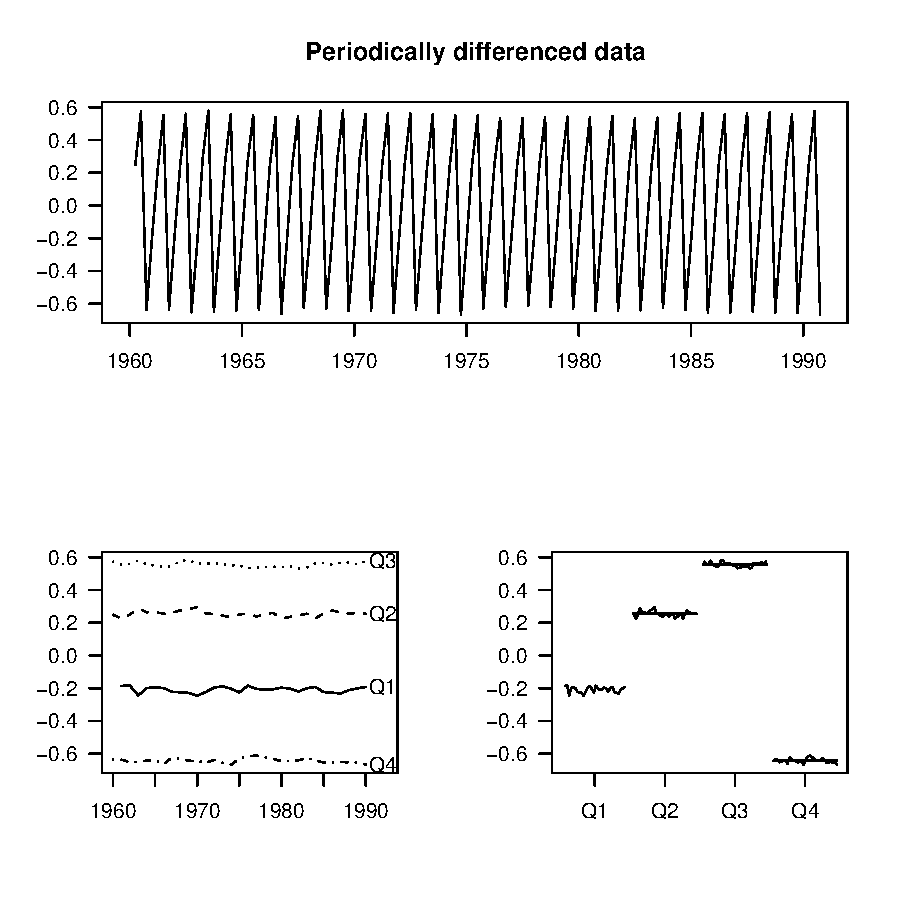
\includegraphics{partsm-pdiffplot}
\end{center}
\end{figure}

For the series \code{lgergnp}, the row with the highest values is the fourth column. This means that the stochastic trend is more likely to undergo changes in the fourth quarter. Reading the impact matrix by columns, the one with the highest is the third column, hence, the third quarter is more sensitive to changes in the stochastic trend.

Obviously, the results above also show that the PIAR model contains a root that is exactly equal to 1 because that is precisely the restriction imposed in the parameters of the model. The other slots of the output not cited here are matrices for internal use when making forecast in a PIAR model.

\subsection[Out-of-sample forecasts]{Out-of-sample forecasts}

The function \code{predictpiar} makes prediction based on PIAR model of order up to 2. By default seasonal intercepts are included. This function computes one-year-ahead forecasting on the basis of the multivariate representation. The forecast for the year $T+$ is $Y_{T+1} = \Phi_0^{-1}\,\mu + \Phi_0^{-1}\,\Phi_1\,Y_T$. The confidence intervals are computed deriving the multivariate moving averages representation from the matrices for the multivariate PIAR model. 

The code below peforms 24 ahead forecasts in the PIAR(2) model. For programming convenience, the number of forescasts, \code{hpred}, must be a multipple of the periodicity of the data. The output of this function provides an object of class \code{pred.piartsm} containing the forecast, the standard errors, the upper and lower 95 per cent confidence bound, as well as the input, i.e., the original data, the order of the model, and the number of predictions.

%%~ Trasladar los resultados a la serie original (sin logaritmos).
\begin{Schunk}
\begin{Sinput}
> out.pred <- predictpiar(wts = lgergnp, p = 2, hpred = 24)
> show(out.pred)
\end{Sinput}
\begin{Soutput}
----
    Forecasts for a PIAR model of order 2 .

           fcast        fse      ucb      lcb
1991.01 6.122634 0.01367962 6.149446 6.095822
1991.02 6.144360 0.01422858 6.172248 6.116472
1991.03 6.157955 0.02203233 6.201138 6.114772
1991.04 6.211668 0.02392443 6.258560 6.164776
1992.01 6.155275 0.02971131 6.213509 6.097041
1992.02 6.175753 0.02791603 6.230469 6.121038
1992.03 6.186578 0.03080442 6.246955 6.126201
1992.04 6.243526 0.03396763 6.310103 6.176950
1993.01 6.187916 0.03867466 6.263719 6.112114
1993.02 6.207147 0.03666874 6.279017 6.135276
1993.03 6.215201 0.03766021 6.289015 6.141387
1993.04 6.275385 0.04165990 6.357038 6.193731
1994.01 6.220557 0.04589664 6.310515 6.130600
1994.02 6.238540 0.04369796 6.324188 6.152892
1994.03 6.243824 0.04344974 6.328985 6.158662
1994.04 6.307243 0.04813840 6.401594 6.212892
1995.01 6.253198 0.05212677 6.355367 6.151030
1995.02 6.269933 0.04974349 6.367431 6.172436
1995.03 6.272447 0.04855385 6.367612 6.177281
1995.04 6.339101 0.05384296 6.444634 6.233569
1996.01 6.285840 0.05768791 6.398908 6.172771
1996.02 6.301327 0.05513000 6.409382 6.193272
1996.03 6.301070 0.05317023 6.405283 6.196856
1996.04 6.370960 0.05899850 6.486597 6.255323

  'fcast': Forecast; 'fse': Forecast standard error; 
  'ucb': Upper confidence bound; 'lcb': Lower condidence bound. 


\end{Soutput}
\end{Schunk}

Remember that the data are scaled in logarithms, hence, for the results to be interpreted, the original scale must be set. The code below makes this task and plots a graphic with the forecast and confidence intervals displayed in Figure \ref{Fpred}.

% Trasladar los resultados a la serie original (sin logaritmos).
\begin{Schunk}
\begin{Sinput}
> out.pred@wts <- exp(1)^out.pred@wts
> out.pred@fcast <- exp(1)^out.pred@fcast
> out.pred@ucb <- exp(1)^out.pred@ucb
> out.pred@lcb <- exp(1)^out.pred@lcb
> plotpredpiar(out.pred)
\end{Sinput}
\end{Schunk}

% <<predplot, fig=TRUE, echo=FALSE, height=4.5, width=5>>=
\begin{figure}[ht]
\begin{center}
\caption{\label{Fpred} Forecast and confidence intervals}
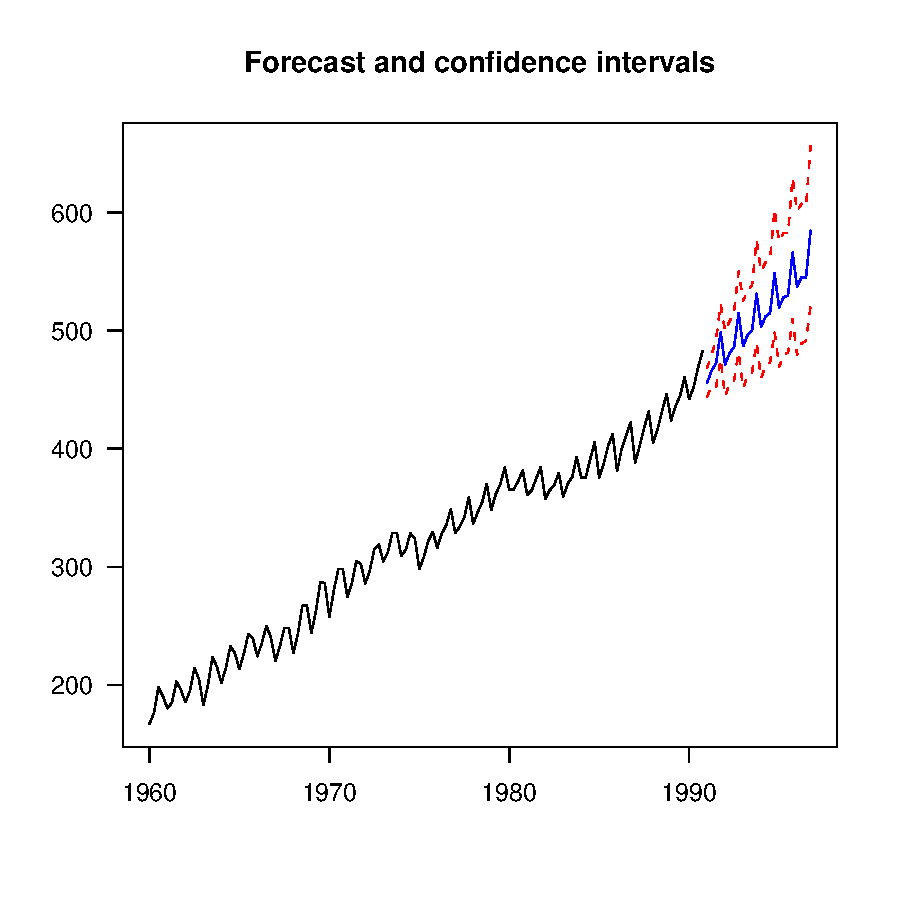
\includegraphics{partsm-predplot}
\end{center}
\end{figure}

\section[Known bugs]{Known bugs} \label{Sbugs}

\begin{itemize}
\item \code{fit.piar} function may give an error message similar to \code{Error in nls(form.rpar, start = nlsinit, trace = FALSE) : step factor 0.000488281 reduced below} $\quad$ \code{'minFactor' of 0.000976562}. The reason for it might be that the initial values selected for performing non-linear least squares are too far from converge. Other alternatives (not available at user level) should be considered for it.
\end{itemize}

If you experiment any bug or pitfalls using \pkg{partsm}, or have some improvement or comment to suggest, please report it to \email{javlacalle@yahoo.es}.

%\section[Concluding remarks]{Concluding remarks} \label{Sconcl}

\clearpage  % tambi�n para meter tablas, figuras dentro de su secci�n
\bibliography{partsm.bib}

\end{document}
